\section{Experimentos}\label{section_experimento}

Como forma de avaliar o modelo proposto serão conduzidos dois principais experimentos.

\subsection{Experimento 1: Formação de assembleias neuronais}

O primeiro experimento consiste em simular a RNP apresentando estímulos ao modelo de retina e analisar se a repetição dos
estímulos leva à formação de assembleias neuronais associadas a cada estímulo a longo prazo. Os estímulos consistem em seis
imagens simples de serem reconhecidas, exibidas na Figura~\ref{fig_estimulos}, e são apresentados à rede de forma intercalada e
aleatória. Quatro estímulos foram reaproveitados do trabalho de~\citeonline{zenkeDiverse2015}, enquanto as figuras de diamante e
de cruz foram adicionadas com o intuito de colocar a RNP mais próxima do seu limite.

\begin{figure}[!ht]
\caption{Os seis estímulos apresentados à RNP durante os experimentos.}
\centering{
\parbox{12cm}{
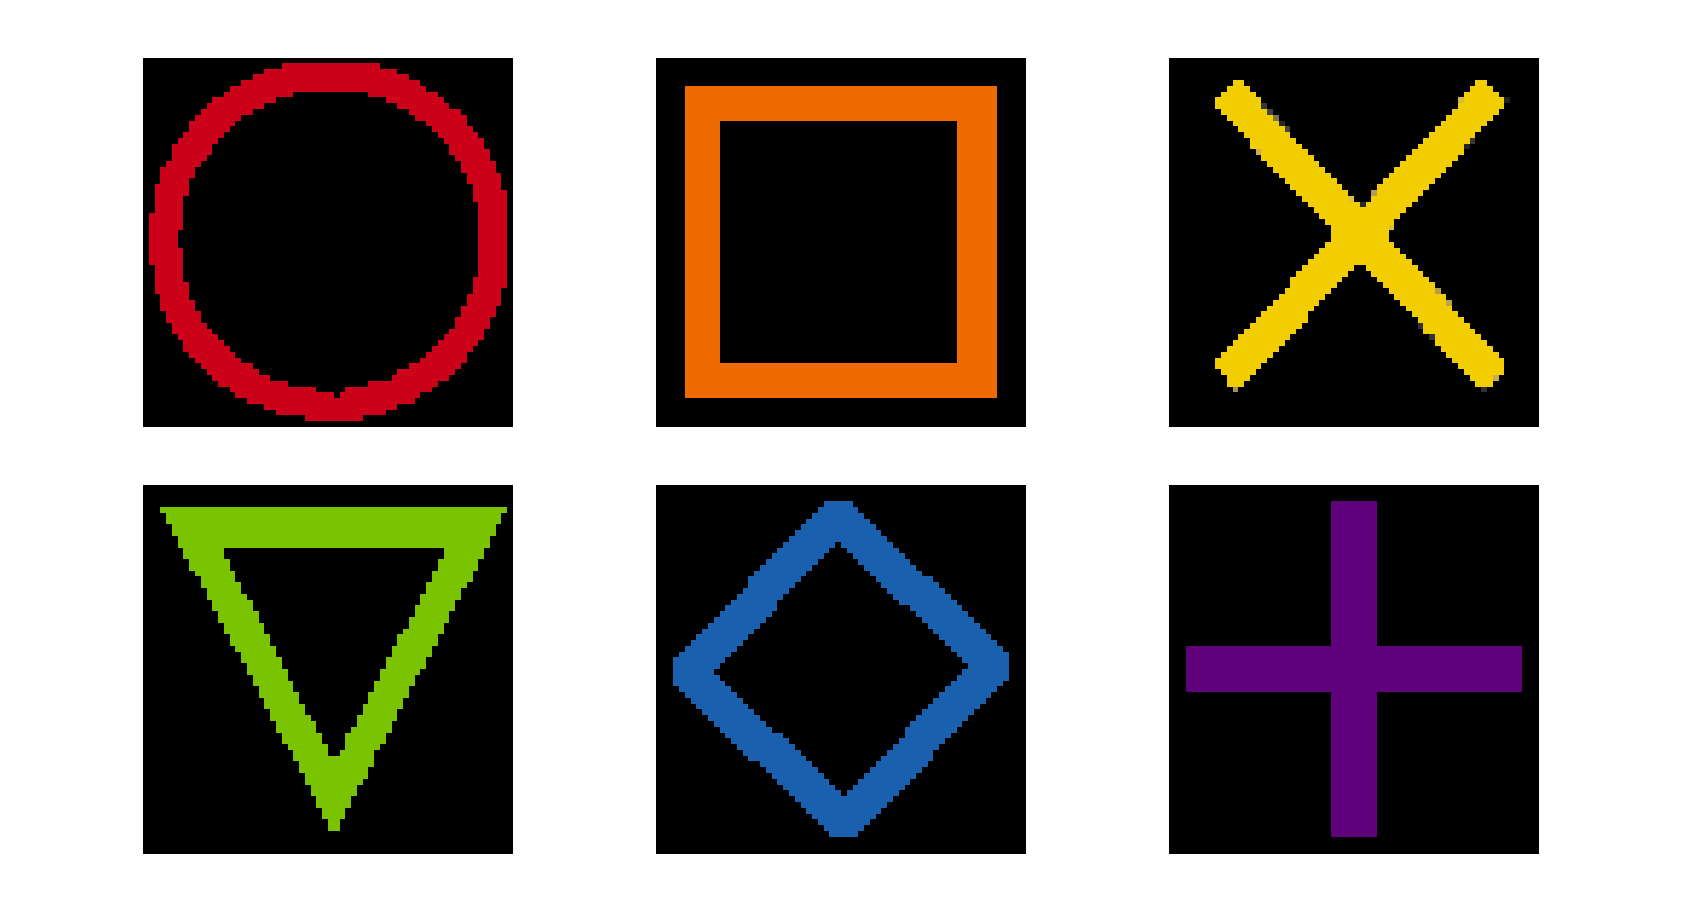
\includegraphics[width=12cm]{figuras/estimulos_cor.png}\label{fig_estimulos}
\fonte{Elaborado pelo autor (2023).}}}
\end{figure}

O objetivo desse experimento é ter uma base de comparação para o experimento 2. Espera-se que a repetição desses
estímulos durante o tempo de simulação da RNP leve à formação de assembleias neuronais associadas a cada estímulo.

\subsection{Experimento 2: Formação de assembleias neuronais com sono}

De forma similar ao experimento 1, o segundo experimento consiste em simular a RNP apresentando os mesmos estímulos, mas dessa vez
com a simulação de sono. O objetivo desse experimento é analisar se a simulação de sono tem algum efeito na formação de
assembleias neuronais. Espera-se que a simulação de sono leve à formação de assembleias neuronais mais rapidamente e que elas
durem mais tempo e sejam mais estáveis, bem como possa permitir o esquecimento de estímulos já não mais relevantes e a memorização
de mais estímulos.

\section{Análise}

A parte final do trabalho consistirá em analisar as diferentes simulações feitas e determinar se a simulação de sono teve algum
efeito na formação de assembleias neuronais. Para isso, antes de tudo é necessário um modo de identificar as assembleias neuronais
e quais neurônios pertencem a cada uma.

Para determinar quais neurônios pertencem à assembleia neuronal associada a um estímulo, será analisada a frequência de disparos de
cada neurônio no intervalo $3s < t < 3.5s$ após a apresentação do estímulo. Os neurônios que disparam com frequência maior que
10Hz serão considerados como pertencentes à assembleia neuronal associada a um estímulo.

Por fim, será analisado quanto tempo leva para a assembleia neuronal associada ser formada e quanto tempo ela dura nas diferentes
simulações.


